\documentclass[11pt,a4paper]{article}

% ── Packages ──────────────────────────────────────────────────────────
\usepackage[utf8]{inputenc}
\usepackage[T1]{fontenc}
\usepackage{lmodern}
\usepackage[margin=1in]{geometry}
\usepackage{amsmath,amssymb,amsthm}
\usepackage{graphicx}
\usepackage{hyperref}
\usepackage{xcolor}
\usepackage{listings}
\usepackage{booktabs}
\usepackage{enumitem}
\usepackage{float}
\usepackage{tikz}
\usetikzlibrary{arrows.meta,positioning,shapes.geometric,calc}
\usepackage{fancyhdr}
\usepackage{titlesec}
\usepackage{caption}
\usepackage{longtable}
\usepackage{tabularx}

% ── Colors ────────────────────────────────────────────────────────────
\definecolor{modblue}{HTML}{1E3A5F}
\definecolor{modcyan}{HTML}{0EA5E9}
\definecolor{codebg}{HTML}{F8F9FA}
\definecolor{codeframe}{HTML}{DEE2E6}
\definecolor{solidity}{HTML}{363636}

% ── Hyperref Setup ────────────────────────────────────────────────────
\hypersetup{
    colorlinks=true,
    linkcolor=modblue,
    citecolor=modblue,
    urlcolor=modcyan,
    pdftitle={MOD Protocol Whitepaper},
    pdfauthor={MOD Protocol},
}

% ── Code Listings ─────────────────────────────────────────────────────
\lstdefinestyle{solidity}{
    backgroundcolor=\color{codebg},
    frame=single,
    rulecolor=\color{codeframe},
    basicstyle=\ttfamily\small,
    keywordstyle=\color{modblue}\bfseries,
    commentstyle=\color{gray},
    stringstyle=\color{teal},
    breaklines=true,
    numbers=left,
    numberstyle=\tiny\color{gray},
    numbersep=8pt,
    tabsize=4,
    showstringspaces=false,
    morekeywords={function,external,internal,public,private,view,pure,returns,
                  require,mapping,address,uint256,uint8,bool,string,memory,
                  calldata,struct,event,emit,modifier,contract,interface,
                  pragma,solidity,import,is},
}

\lstdefinestyle{python}{
    backgroundcolor=\color{codebg},
    frame=single,
    rulecolor=\color{codeframe},
    basicstyle=\ttfamily\small,
    keywordstyle=\color{modblue}\bfseries,
    commentstyle=\color{gray},
    stringstyle=\color{teal},
    breaklines=true,
    numbers=left,
    numberstyle=\tiny\color{gray},
    numbersep=8pt,
    tabsize=4,
    showstringspaces=false,
    language=Python,
}

% ── Header/Footer ────────────────────────────────────────────────────
\pagestyle{fancy}
\fancyhf{}
\fancyhead[L]{\small\textcolor{gray}{MOD Protocol Whitepaper}}
\fancyhead[R]{\small\textcolor{gray}{v1.0 -- March 2026}}
\fancyfoot[C]{\thepage}
\renewcommand{\headrulewidth}{0.4pt}

% ── Title Formatting ─────────────────────────────────────────────────
\titleformat{\section}{\Large\bfseries\color{modblue}}{\thesection}{1em}{}
\titleformat{\subsection}{\large\bfseries\color{modblue!80}}{\thesubsection}{1em}{}
\titleformat{\subsubsection}{\normalsize\bfseries\color{modblue!60}}{\thesubsubsection}{1em}{}

% ── Theorem Environments ─────────────────────────────────────────────
\newtheorem{definition}{Definition}[section]
\newtheorem{property}{Property}[section]

% ══════════════════════════════════════════════════════════════════════
\begin{document}

% ── Title Page ────────────────────────────────────────────────────────
\begin{titlepage}
\centering
\vspace*{3cm}

{\Huge\bfseries\textcolor{modblue}{MOD Protocol}\par}
\vspace{0.5cm}
{\Large\textcolor{gray}{A Decentralized Modular Development Framework\\with Time-Weighted Revenue Distribution}\par}

\vspace{2cm}

{\large Version 1.0\par}
{\large March 2026\par}

\vspace{3cm}

\begin{abstract}
\noindent
We present MOD Protocol, a decentralized modular development framework that unifies on-chain economic primitives with off-chain composable computation. The protocol introduces \emph{BlocTime}---a time-weighted staking mechanism that distributes real marketplace revenue to long-term participants proportional to their lock commitment. MOD operates across a five-layer architecture: a Python framework core with 174 composable orbit modules, a BlocTime smart contract suite deployed on Base (EVM), a FastAPI service layer, IPFS-backed distributed storage, and a Next.js frontend. Developers register callable functions on-chain, set prices, and earn revenue each time their modules are invoked. Revenue flows through a Treasury contract and is distributed to BlocTime stakers without inflationary token emission. All core contracts implement a \texttt{setOwnerless()} function enabling irreversible decentralization. The protocol supports multi-chain operation across EVM, Substrate, and Solana ecosystems.
\end{abstract}

\vfill
\end{titlepage}

% ── Table of Contents ─────────────────────────────────────────────────
\tableofcontents
\newpage

% ══════════════════════════════════════════════════════════════════════
\section{Introduction}
\label{sec:introduction}

\subsection{Problem Statement}

Modern software development relies on composable libraries and microservices, yet developers receive no direct economic benefit when their code is consumed by others at runtime. Package registries (npm, PyPI) track downloads but provide no revenue mechanism. Existing blockchain-based marketplaces either (a)~require developers to learn Solidity and smart contract development, (b)~operate inflationary token models divorced from real economic activity, or (c)~lack the composability needed for general-purpose software engineering.

\subsection{Solution}

MOD Protocol bridges the gap between on-chain economics and off-chain development by providing:

\begin{enumerate}[label=\arabic*.]
    \item \textbf{Zero-friction module registration}: Developers drop a Python module into the orbit directory; the framework auto-discovers it with no configuration required.
    \item \textbf{On-chain revenue flow}: Module invocations generate fees that accumulate in a Treasury contract and are distributed to stakers.
    \item \textbf{Time-weighted staking}: The BlocTime mechanism rewards long-term commitment through a configurable multiplier curve.
    \item \textbf{Non-inflationary rewards}: All staker rewards derive from real marketplace activity (credit fees, debit fees), not token minting.
    \item \textbf{Irreversible decentralization}: Every core contract includes \texttt{setOwnerless()}, a one-way function that permanently renounces administrative control.
\end{enumerate}

\subsection{Design Principles}

\begin{itemize}
    \item \textbf{Composability over monolithism}: 174 independent modules that compose at runtime.
    \item \textbf{Revenue from usage, not inflation}: Treasury rewards funded exclusively by marketplace fees.
    \item \textbf{Progressive decentralization}: Contracts begin owner-managed, with an irreversible path to full decentralization.
    \item \textbf{Multi-chain by default}: Native support for EVM (Base, Ethereum, Polygon), Substrate (Polkadot), and Solana.
\end{itemize}

% ══════════════════════════════════════════════════════════════════════
\section{Protocol Architecture}
\label{sec:architecture}

\subsection{Five-Layer Stack}

\begin{figure}[H]
\centering
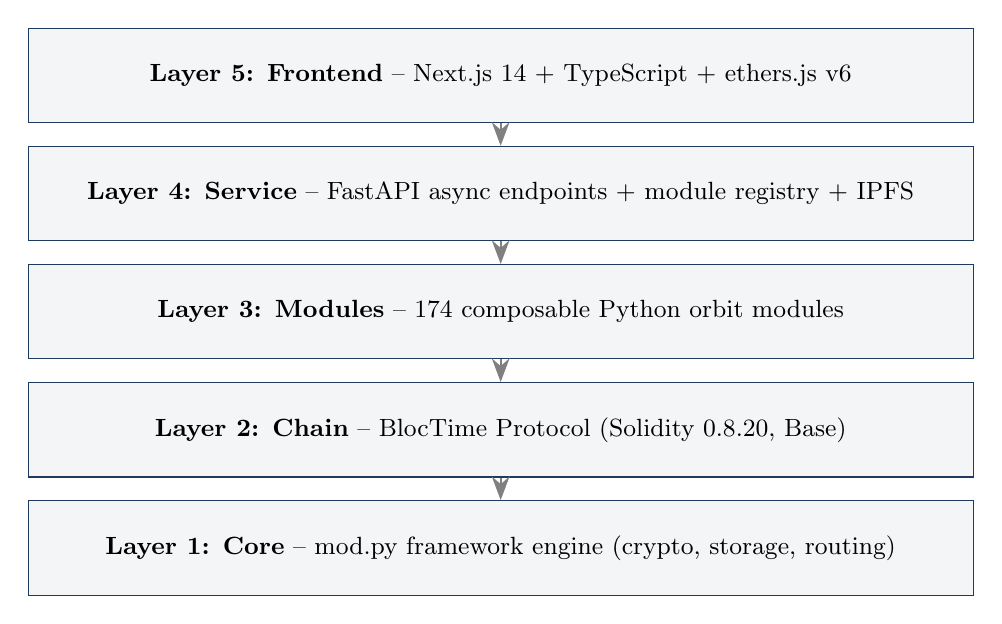
\begin{tikzpicture}[
    layer/.style={rectangle, draw=modblue, fill=modblue!5, minimum width=12cm, minimum height=1.2cm, font=\small},
    arrow/.style={-{Stealth[length=3mm]}, thick, gray}
]
    \node[layer] (L5) at (0,5)   {\textbf{Layer 5: Frontend} -- Next.js 14 + TypeScript + ethers.js v6};
    \node[layer] (L4) at (0,3.5) {\textbf{Layer 4: Service} -- FastAPI async endpoints + module registry + IPFS};
    \node[layer] (L3) at (0,2)   {\textbf{Layer 3: Modules} -- 174 composable Python orbit modules};
    \node[layer] (L2) at (0,0.5) {\textbf{Layer 2: Chain} -- BlocTime Protocol (Solidity 0.8.20, Base)};
    \node[layer] (L1) at (0,-1)  {\textbf{Layer 1: Core} -- mod.py framework engine (crypto, storage, routing)};

    \draw[arrow] (L5) -- (L4);
    \draw[arrow] (L4) -- (L3);
    \draw[arrow] (L3) -- (L2);
    \draw[arrow] (L2) -- (L1);
\end{tikzpicture}
\caption{MOD Protocol five-layer architecture}
\label{fig:layers}
\end{figure}

\subsection{Data Flow}

The protocol operates a circular economic flow:

\begin{enumerate}
    \item \textbf{Developer} registers a module on-chain via \texttt{Registry.sol}, uploads code to IPFS, and sets a price in the module configuration.
    \item \textbf{User} discovers the module, deposits stablecoins into \texttt{Market.sol} (credit operation), and invokes the module function (debit operation).
    \item \textbf{Fee split}: 5\% of debit transactions and 1\% of credit transactions flow to the Treasury.
    \item \textbf{Staker} locks NativeToken in \texttt{BlocTime.sol}, receives time-weighted BlocTime tokens, and claims a proportional share of Treasury revenue.
\end{enumerate}

\subsection{Core Framework: mod.py}

The framework engine (\texttt{mod/core/mod.py}, $\sim$1800 lines of code) provides the following subsystems:

\begin{table}[H]
\centering
\begin{tabularx}{\textwidth}{lX}
\toprule
\textbf{Subsystem} & \textbf{Description} \\
\midrule
Module Discovery & Anchor-file pattern: \texttt{agent.py} $>$ \texttt{mod.py} $>$ \texttt{block.py} $>$ \texttt{\{name\}.py} \\
Cryptographic Primitives & ECDSA key generation, AES-256 encryption, signature verification \\
Storage & Encrypted key-value store at \texttt{\textasciitilde/.mod/\{module\}/} \\
Server Management & Process lifecycle for API servers per module \\
Git Integration & Commit, push, repository discovery \\
AI Integration & Claude API for code generation, analysis, refactoring \\
Execution & Thread/process pool executors with function-level caching \\
\bottomrule
\end{tabularx}
\caption{Core framework subsystems}
\end{table}

Module loading is lazy and $O(1)$:

\begin{lstlisting}[style=python]
m.mod('agent')()           # Load module class
m.fn('agent/run')(q='.')   # Call module function directly
\end{lstlisting}

% ══════════════════════════════════════════════════════════════════════
\section{BlocTime Smart Contract Suite}
\label{sec:contracts}

All contracts are compiled with Solidity 0.8.20, use OpenZeppelin libraries, and are deployed on Base Sepolia (Chain ID: 84532).

\subsection{Contract Addresses (Base Sepolia)}

\begin{table}[H]
\centering
\begin{tabularx}{\textwidth}{llX}
\toprule
\textbf{Contract} & \textbf{Address} & \textbf{Role} \\
\midrule
NativeToken & \texttt{0xB9b6...b51} & Stakeable ERC20 \\
BlocTime & \texttt{0xF25A...bD} & Time-weighted staking \\
Treasury & \texttt{0xe9a9...85} & Revenue distribution \\
Market & \texttt{0x2F0B...87} & Stablecoin marketplace \\
Registry & \texttt{0x4f9e...43} & Module registration \\
Debit & \texttt{0x6F94...42} & EIP-712 signed debits \\
TokenGate & \texttt{0x97c7...8b} & Whitelist \& oracle registry \\
ManualPriceOracle & \texttt{0x40C3...F1} & Price feeds \\
USDC & \texttt{0xe229...01} & Test stablecoin \\
USDT & \texttt{0xc68d...Bc} & Test stablecoin \\
\bottomrule
\end{tabularx}
\caption{Deployed contract addresses on Base Sepolia}
\end{table}

\subsection{BlocTime.sol --- Time-Weighted Staking}

\subsubsection{Multiplier Curve}

\begin{definition}[Multiplier Function]
The multiplier function $M: \mathbb{N} \to \mathbb{R}^+$ is defined as a piecewise-linear interpolation over a monotonically increasing set of control points $\{(b_i, m_i)\}_{i=0}^{n-1}$:
\begin{equation}
M(x) = \begin{cases}
m_0 & \text{if } x \leq b_0 \\[6pt]
m_i + \dfrac{(m_{i+1} - m_i)(x - b_i)}{b_{i+1} - b_i} & \text{if } b_i < x \leq b_{i+1} \\[6pt]
m_{n-1} & \text{if } x > b_{n-1}
\end{cases}
\label{eq:multiplier}
\end{equation}
where $b_i$ is measured in blocks and $m_i$ in basis points ($10000 = 1.0\times$).
\end{definition}

\begin{property}[Monotonicity]
The control points satisfy strict monotonicity in block count and weak monotonicity in multiplier:
\begin{equation}
b_i < b_{i+1} \quad \text{and} \quad m_i \leq m_{i+1} \quad \forall\, i \in \{0, \ldots, n-2\}
\end{equation}
This is enforced on-chain during \texttt{setPoints()} to prevent gaming via non-monotonic curves.
\end{property}

\begin{table}[H]
\centering
\begin{tabular}{cc}
\toprule
\textbf{Lock Duration (blocks)} & \textbf{Multiplier} \\
\midrule
0 & $1.0\times$ (10000 bps) \\
10{,}000 & $1.5\times$ (15000 bps) \\
50{,}000 & $2.0\times$ (20000 bps) \\
100{,}000 & $3.0\times$ (30000 bps) \\
\bottomrule
\end{tabular}
\caption{Example multiplier curve configuration}
\end{table}

\subsubsection{Staking Mechanics}

\begin{lstlisting}[style=solidity]
function stake(uint256 amount, uint256 lockBlocks) external {
    require(amount > 0);
    require(lockBlocks <= maxLockBlocks);
    token.transferFrom(msg.sender, address(this), amount);
    uint256 bloctime = amount * getMultiplier(lockBlocks) / 10000;
    _mint(msg.sender, bloctime);
    positions[msg.sender][nextId] = StakePosition({
        amount: amount,
        lockBlocks: lockBlocks,
        startBlock: block.number,
        bloctimeMinted: bloctime
    });
}

function unstake(uint256 stakeId) external {
    StakePosition storage pos = positions[msg.sender][stakeId];
    require(block.number >= pos.startBlock + pos.lockBlocks);
    _burn(msg.sender, pos.bloctimeMinted);
    token.transfer(msg.sender, pos.amount);
}
\end{lstlisting}

Multiple concurrent positions per address are supported, each with an independent lock schedule.

\subsection{Treasury.sol --- Multi-Token Revenue Distribution}

\subsubsection{Distribution Formula}

\begin{definition}[Claimable Amount]
For a holder with governance token balance $g_u$, total governance supply $G$, treasury balance $T_k$ of token $k$, and owner percentage $p$ (in basis points):
\begin{equation}
\text{claimable}_{u,k} = \frac{T_k \cdot (10000 - p) \cdot g_u}{10000 \cdot G}
\label{eq:treasury}
\end{equation}
\end{definition}

The calculation uses current balances (snapshot-free), avoiding the gas overhead of historical accounting. The governance token is BlocTime, making the distribution proportional to time-weighted stake commitment.

\subsubsection{Multi-Token Support}

The Treasury accepts any ERC20 token whitelisted through TokenGate. The \texttt{withdrawAll()} function iterates over all whitelisted tokens and transfers the caller's proportional share of each.

\subsection{Market.sol --- Stablecoin Marketplace}

\subsubsection{Credit (Deposit)}

\begin{lstlisting}[style=solidity]
function credit(
    address paymentToken,
    uint256 stableAmount,
    uint256 maxPaymentAmount
) external nonReentrant whenNotPaused {
    (uint256 price, uint8 decimals,) = oracle.getPrice(paymentToken);
    uint256 paymentAmount = stableAmount * price / (10 ** decimals);
    uint256 fee = paymentAmount * creditFeeBps / 10000;
    paymentToken.safeTransferFrom(msg.sender, treasury, fee);
    paymentToken.safeTransferFrom(msg.sender, address(this),
                                  paymentAmount - fee);
    uint256 minted = stableAmount * (10000 - creditFeeBps) / 10000;
    _mint(msg.sender, minted);
}
\end{lstlisting}

\subsubsection{Withdrawal (Instant)}

\begin{lstlisting}[style=solidity]
function withdraw(
    address paymentToken,
    uint256 stableAmount,
    uint256 minReceiveAmount
) external nonReentrant {
    _burn(msg.sender, stableAmount);
    (uint256 price, uint8 decimals,) = oracle.getPrice(paymentToken);
    uint256 paymentAmount = stableAmount * price / (10 ** decimals);
    require(paymentAmount >= minReceiveAmount, "Slippage exceeded");
    paymentToken.safeTransfer(msg.sender, paymentAmount);
}
\end{lstlisting}

Key properties: no lockup period, instant liquidity, 0.1\% withdrawal fee, slippage protection via \texttt{minReceiveAmount}.

\subsection{Registry.sol --- On-Chain Module Registration}

Modules are registered with a unique \texttt{(creator, name)} tuple and arbitrary metadata (typically an IPFS CID):

\begin{lstlisting}[style=solidity]
function registerMod(string memory name, string memory data)
    external returns (uint256 modId);
function updateMod(uint256 modId, string memory data) external;
function removeMod(uint256 modId) external;
function transferOwnership(uint256 modId, address newOwner) external;
function getUserMods(address user) external view returns (uint256[] memory);
\end{lstlisting}

\subsection{Perms.sol --- Hierarchical Key-Based Access Control}

A generic permission system mapping parent keys to arrays of child keys:

\begin{itemize}
    \item First caller to \texttt{addKey(parent, child)} becomes the owner of that parent key.
    \item Owner can \texttt{setKeys()}, \texttt{removeKey()}, \texttt{transferKeyOwnership()}.
    \item Configurable limits: max child keys (default 100), max key size (default 1024 bytes).
    \item Swap-and-pop deletion for $O(1)$ removal.
\end{itemize}

% ══════════════════════════════════════════════════════════════════════
\section{Tokenomics \& Economic Model}
\label{sec:tokenomics}

\subsection{Token Taxonomy}

\begin{table}[H]
\centering
\begin{tabularx}{\textwidth}{llclX}
\toprule
\textbf{Token} & \textbf{Type} & \textbf{Decimals} & \textbf{Supply} & \textbf{Purpose} \\
\midrule
NativeToken & ERC20 & 18 & Fixed (minted on deploy) & Stakeable governance asset \\
BlocTime & ERC20 & 18 & Dynamic (mint/burn) & Time-weighted stake receipt \\
Market Token & ERC20 & 8 & Dynamic (mint/burn) & USD-pegged marketplace credit \\
USDC / USDT & ERC20 & 6 & External & Payment tokens \\
\bottomrule
\end{tabularx}
\caption{Token taxonomy}
\end{table}

\subsection{Value Flow}

\begin{figure}[H]
\centering
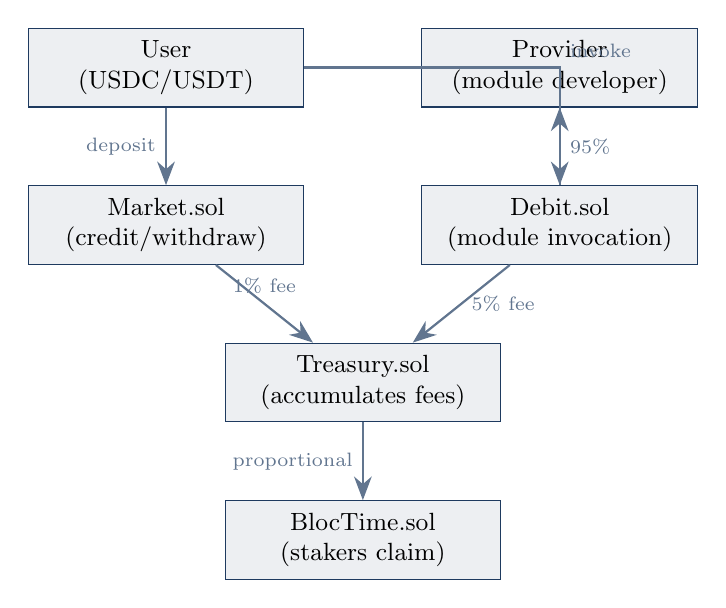
\begin{tikzpicture}[
    box/.style={rectangle, draw=modblue, fill=modblue!8, minimum width=3.5cm, minimum height=1cm, align=center, font=\small},
    arrow/.style={-{Stealth[length=3mm]}, thick, modblue!70},
    fee/.style={font=\scriptsize\color{red!70!black}}
]
    % Nodes
    \node[box] (user) at (0,4) {User\\(USDC/USDT)};
    \node[box] (market) at (0,2) {Market.sol\\(credit/withdraw)};
    \node[box] (debit) at (5,2) {Debit.sol\\(module invocation)};
    \node[box] (treasury) at (2.5,0) {Treasury.sol\\(accumulates fees)};
    \node[box] (staking) at (2.5,-2) {BlocTime.sol\\(stakers claim)};
    \node[box] (provider) at (5,4) {Provider\\(module developer)};

    % Arrows
    \draw[arrow] (user) -- node[left, fee] {deposit} (market);
    \draw[arrow] (market) -- node[above, fee] {1\% fee} (treasury);
    \draw[arrow] (user) -| node[above right, fee] {invoke} (debit);
    \draw[arrow] (debit) -- node[right, fee] {5\% fee} (treasury);
    \draw[arrow] (debit) -- node[right, fee] {95\%} (provider);
    \draw[arrow] (treasury) -- node[left, fee] {proportional} (staking);
\end{tikzpicture}
\caption{Economic value flow through the protocol}
\label{fig:valueflow}
\end{figure}

\subsection{Fee Schedule}

\begin{table}[H]
\centering
\begin{tabular}{llll}
\toprule
\textbf{Operation} & \textbf{Fee Rate} & \textbf{Destination} & \textbf{Mechanism} \\
\midrule
Market Credit & 1\% (configurable, bps) & Treasury & Automatic on \texttt{credit()} \\
Market Withdrawal & 0.1\% & Retained in Market & Implicit in conversion \\
Debit Execution & 5\% (constant) & Treasury & Automatic on \texttt{executeDebit()} \\
Owner Claim & Configurable \% & Owner address & Manual via \texttt{ownerWithdraw()} \\
\bottomrule
\end{tabular}
\caption{Protocol fee schedule}
\end{table}

\subsection{Staking Reward Derivation}

Let:
\begin{itemize}
    \item $S_u$ = user's staked NativeToken amount
    \item $L_u$ = user's chosen lock duration (blocks)
    \item $M(L_u)$ = multiplier at lock duration $L_u$ (basis points, per Equation~\ref{eq:multiplier})
    \item $B_u = S_u \cdot M(L_u) / 10000$ = user's BlocTime balance
    \item $B_{\text{total}} = \sum_{i} B_i$ = total BlocTime supply
    \item $T_k$ = Treasury balance of token $k$
    \item $p$ = owner percentage (basis points)
\end{itemize}

\begin{definition}[User Reward]
The claimable amount for user $u$ of token $k$:
\begin{equation}
R_{u,k} = \frac{T_k \cdot (10000 - p)}{10000} \cdot \frac{B_u}{B_{\text{total}}}
\label{eq:reward}
\end{equation}
\end{definition}

\begin{definition}[Annualized Yield]
Assuming constant Treasury inflow rate $F_k$ per year:
\begin{equation}
\text{APY}_{u,k} = \frac{F_k \cdot (10000 - p)}{10000} \cdot \frac{M(L_u)}{P_{\text{native}} \cdot B_{\text{total}}} \times 100\%
\label{eq:apy}
\end{equation}
where $P_{\text{native}}$ is the NativeToken price in token $k$ terms.
\end{definition}

\subsection{Anti-Gaming Properties}

\begin{property}[Flash Loan Resistance]
BlocTime tokens can only be minted by staking NativeToken with a lock period $L_u > 0$ blocks. Since the lock enforces that tokens cannot be unstaked in the same block, flash-loan attacks on the Treasury distribution are structurally infeasible---an attacker cannot acquire BlocTime, claim, and exit within a single transaction.
\end{property}

\begin{property}[Multiplier Monotonicity]
The monotonic constraint on control points ($m_i \leq m_{i+1}$) prevents arbitrage between lock durations. A rational actor always maximizes BlocTime per unit staked by choosing the longest lock they can tolerate.
\end{property}

\begin{property}[Non-Inflationary Supply]
The NativeToken has a fixed supply minted at deployment. BlocTime is minted and burned symmetrically via stake/unstake. Market tokens are backed 1:1 by deposited stablecoins. No mechanism exists to create unbacked tokens.
\end{property}

% ══════════════════════════════════════════════════════════════════════
\section{Module System \& Orbit Ecosystem}
\label{sec:modules}

\subsection{Module Structure}

Every orbit module follows a canonical directory layout:

\begin{lstlisting}[basicstyle=\ttfamily\small, frame=single, backgroundcolor=\color{codebg}]
mod/orbit/{module_name}/
  {module_name}/
    mod.py              # Primary anchor file
    __init__.py
    requirements.txt    # Python dependencies
    config.json         # Module configuration
    README.md           # Documentation
\end{lstlisting}

Anchor file resolution order: \texttt{agent.py} $>$ \texttt{mod.py} $>$ \texttt{block.py} $>$ \texttt{\{name\}.py}.

\subsection{Module Categories (174 total)}

\begin{table}[H]
\centering
\begin{tabularx}{\textwidth}{lcX}
\toprule
\textbf{Category} & \textbf{Count} & \textbf{Key Modules} \\
\midrule
AI \& Agents & 6 & \texttt{agent}, \texttt{claude}, \texttt{model}, \texttt{model.openrouter}, \texttt{skill} \\
Storage \& Data & 5 & \texttt{ipfs}, \texttt{filecoin}, \texttt{lighthouse}, \texttt{cache}, \texttt{localfs} \\
Blockchain \& DeFi & 8 & \texttt{bridge}, \texttt{uniswap}, \texttt{safe}, \texttt{eth}, \texttt{near}, \texttt{solana}, \texttt{raydium} \\
Dev Tools & 6 & \texttt{git}, \texttt{gitagent}, \texttt{pytest}, \texttt{conda}, \texttt{docker} \\
Infrastructure & 149+ & \texttt{web}, \texttt{mcp}, \texttt{modal}, \texttt{registry}, \texttt{perms}, \texttt{ssh} \\
\bottomrule
\end{tabularx}
\caption{Orbit module ecosystem}
\end{table}

\subsection{Module Lifecycle}

\begin{enumerate}
    \item \textbf{Discover}: \texttt{mod.py} scans \texttt{orbit/} for anchor files ($O(n)$ at startup, cached).
    \item \textbf{Load}: \texttt{m.mod('name')} imports and instantiates (lazy, $O(1)$).
    \item \textbf{Register}: \texttt{api.reg('name')} uploads to IPFS + writes to \texttt{Registry.sol}.
    \item \textbf{Invoke}: \texttt{m.fn('name/function')(args)} executes locally.
    \item \textbf{Monetize}: Remote calls route through Market $\to$ Debit $\to$ fee to Treasury.
\end{enumerate}

\subsection{IPFS-Backed Registry}

Module metadata is stored on IPFS (Kubo v0.40.1 daemon, auto-managed). Versioning is achieved by updating the CID pointer on-chain; previous CIDs remain accessible on IPFS indefinitely:

\begin{lstlisting}[style=python]
# Registration flow
cid = ipfs.put(module_code_and_metadata)
registry.registerMod(name, cid)   # On-chain pointer

# Retrieval flow
(owner, name, cid) = registry.getMod(modId)
metadata = ipfs.get(cid)
\end{lstlisting}

% ══════════════════════════════════════════════════════════════════════
\section{On-Chain Registry \& Marketplace}
\label{sec:marketplace}

\subsection{Registration}

\begin{lstlisting}[style=solidity]
function registerMod(string memory name, string memory data)
    external returns (uint256 modId)
\end{lstlisting}

\begin{itemize}
    \item \texttt{name}: Human-readable identifier, unique per \texttt{(msg.sender, name)} tuple.
    \item \texttt{data}: Arbitrary string (IPFS CID, JSON, or URI).
    \item Returns: Monotonically increasing \texttt{modId}.
\end{itemize}

\subsection{Market Credit/Withdraw Cycle}

The credit operation converts stablecoins into USD-pegged Market tokens (1\% fee to Treasury). The withdraw operation burns Market tokens and returns stablecoins instantly with 0.1\% fee. Slippage protection is enforced on both operations.

\subsection{Module Invocation Payment}

When a user invokes a paid module:
\begin{enumerate}
    \item User calls \texttt{Debit.executeDebit(client, provider, amount, deadline, signature)}.
    \item Debit contract verifies EIP-712 signature and authority approvals.
    \item 5\% fee transferred to Treasury.
    \item 95\% transferred to provider.
    \item Provider's module executes the function.
\end{enumerate}

% ══════════════════════════════════════════════════════════════════════
\section{Oracle System \& Price Feeds}
\label{sec:oracle}

\subsection{Architecture}

The oracle system uses a pluggable adapter pattern:

\begin{lstlisting}[style=solidity]
interface IOracleAdapter {
    function getPrice(address token)
        external view returns (uint256 price, uint8 decimals, uint256 timestamp);
    function hasPriceFeed(address token)
        external view returns (bool);
}
\end{lstlisting}

Three adapter implementations are provided:
\begin{itemize}
    \item \textbf{ManualPriceOracle}: Owner-set prices for development and testing.
    \item \textbf{ChainlinkAdapter}: Integration with Chainlink decentralized price feeds.
    \item \textbf{PythAdapter}: Integration with Pyth Network high-frequency feeds.
\end{itemize}

\subsection{Price Resolution}

\texttt{TokenGate} resolves prices with a fallback chain:
\begin{enumerate}
    \item Check token-specific oracle $\to$ if registered and has feed, use it.
    \item Fall back to default oracle $\to$ if set.
    \item Revert if no oracle available.
\end{enumerate}

% ══════════════════════════════════════════════════════════════════════
\section{Debit Protocol \& EIP-712 Authorization}
\label{sec:debit}

\subsection{EIP-712 Domain}

\begin{lstlisting}[style=solidity]
EIP712Domain({
    name: "ModDebit",
    version: "1",
    chainId: <chain_id>,
    verifyingContract: <Debit_address>
})
\end{lstlisting}

\subsection{Authorization Structure}

\begin{lstlisting}[style=solidity]
struct DebitAuthorization {
    address client;       // Who is being debited
    address provider;     // Who receives payment
    uint256 amount;       // Stable amount
    uint256 nonce;        // Replay prevention
    uint256 deadline;     // Signature expiry (block.timestamp)
}
\end{lstlisting}

\subsection{Multi-Authority Approval System}

Clients can configure a multi-signature approval scheme:
\begin{enumerate}
    \item \textbf{Add authorities}: \texttt{addAuthority(address)} --- trusted approvers.
    \item \textbf{Set threshold}: \texttt{setApprovalThreshold(n)} --- minimum approvals needed.
    \item \textbf{Authority approves}: \texttt{approveDebit(client, maxAmount, deadline)} --- spending cap + time limit.
    \item \textbf{Execute}: If enough authorities have approved with sufficient remaining allowance.
\end{enumerate}

\subsection{Daily Spending Limits}

Each client has a configurable daily limit (default: 1000 USD equivalent). The limit resets every 86400 seconds. Debits exceeding the remaining daily allowance are reverted.

% ══════════════════════════════════════════════════════════════════════
\section{Security Model}
\label{sec:security}

\subsection{Smart Contract Security}

\begin{table}[H]
\centering
\begin{tabularx}{\textwidth}{lX}
\toprule
\textbf{Measure} & \textbf{Implementation} \\
\midrule
Reentrancy protection & \texttt{ReentrancyGuard} on all state-changing functions \\
Safe token transfers & OpenZeppelin \texttt{SafeERC20} throughout \\
Overflow protection & Solidity 0.8.20 built-in checked arithmetic \\
Access control & \texttt{Ownable} + per-function modifiers \\
Emergency stops & \texttt{Pausable} on Market contract \\
Input validation & \texttt{require} guards on all external functions \\
Monotonic enforcement & Multiplier curve points must be strictly increasing \\
\bottomrule
\end{tabularx}
\caption{Smart contract security measures}
\end{table}

\subsection{Cryptographic Security}

\begin{itemize}
    \item \textbf{Key management}: ECDSA (secp256k1) and Sr25519 key generation.
    \item \textbf{Storage encryption}: AES-256 for sensitive data at rest.
    \item \textbf{Signature verification}: EIP-712 structured data signing for debit authorizations.
    \item \textbf{Safe multisig}: Gnosis Safe integration with $v + 4$ adjustment for \texttt{eth\_sign} mode.
\end{itemize}

\subsection{Anti-Flash-Loan Design}

The Treasury distribution uses current token balances. Since BlocTime can only be minted by staking NativeToken with a lock period, flash-loan attacks on the distribution are structurally infeasible: an attacker cannot acquire, claim, and exit within a single transaction.

% ══════════════════════════════════════════════════════════════════════
\section{Governance \& Decentralization Path}
\label{sec:governance}

\subsection{Ownership Model}

All core contracts inherit \texttt{Ownable} with an additional \texttt{setOwnerless()} function:

\begin{lstlisting}[style=solidity]
bool public ownerless;

function setOwnerless() external onlyOwner {
    ownerless = true;
    renounceOwnership();
}

modifier notOwnerless() {
    require(!ownerless, "Contract is ownerless");
    _;
}
\end{lstlisting}

This is a \textbf{one-way function}: once called, no administrative changes can ever be made. The \texttt{ownerless} flag is permanent and cannot be reversed.

\subsection{Progressive Decentralization Roadmap}

\begin{table}[H]
\centering
\begin{tabularx}{\textwidth}{lX}
\toprule
\textbf{Phase} & \textbf{Description} \\
\midrule
Phase 1: Managed & Owner = deployer EOA. Full administrative control for rapid iteration. \\
Phase 2: Multisig & Transfer ownership to Gnosis Safe. N-of-M signature requirement. \\
Phase 3: DAO & Governance token voting (BlocTime-weighted). On-chain proposals. \\
Phase 4: Ownerless & \texttt{setOwnerless()} on all contracts. Permanent, irreversible decentralization. \\
\bottomrule
\end{tabularx}
\caption{Progressive decentralization roadmap}
\end{table}

\subsection{Functions Locked by setOwnerless()}

\begin{table}[H]
\centering
\begin{tabularx}{\textwidth}{lX}
\toprule
\textbf{Contract} & \textbf{Locked Functions} \\
\midrule
BlocTime & \texttt{setPoints()}, \texttt{setParams()}, \texttt{emergencyWithdraw()} \\
Treasury & \texttt{setOwnerPercentage()}, \texttt{setGovernanceToken()}, \texttt{setTokenGate()} \\
Market & \texttt{setTreasury()}, \texttt{setTokenGate()}, \texttt{setDebitContract()}, \texttt{pause()}/\texttt{unpause()} \\
Debit & \texttt{setMarket()}, \texttt{setSignatureRequired()} \\
TokenGate & Oracle management, token whitelisting \\
Perms & \texttt{setMaxChildKeys()}, \texttt{setMaxKeySize()} \\
\bottomrule
\end{tabularx}
\caption{Administrative functions permanently locked by \texttt{setOwnerless()}}
\end{table}

% ══════════════════════════════════════════════════════════════════════
\section{Network Deployment}
\label{sec:deployment}

\subsection{Supported Networks}

\begin{table}[H]
\centering
\begin{tabular}{llll}
\toprule
\textbf{Network} & \textbf{Chain ID} & \textbf{Status} & \textbf{RPC} \\
\midrule
Base Sepolia & 84532 & Deployed & \texttt{https://sepolia.base.org} \\
Base Mainnet & 8453 & Production-ready & \texttt{https://mainnet.base.org} \\
Ganache (local) & 1337 & Development & \texttt{localhost:8545} \\
\bottomrule
\end{tabular}
\caption{Supported network configurations}
\end{table}

\subsection{Compiler \& Framework}

\begin{itemize}
    \item \textbf{Solidity}: 0.8.20
    \item \textbf{Framework}: Hardhat
    \item \textbf{Libraries}: OpenZeppelin Contracts v5.x
    \item \textbf{Testing}: Hardhat + Chai (100+ test cases)
\end{itemize}

\subsection{Multi-Chain Module Support}

Beyond EVM contracts, the orbit module ecosystem supports:
\begin{itemize}
    \item \textbf{Substrate}: \texttt{bridge} module (Sr25519 signatures, cross-chain minting via \texttt{BridgeableToken.sol}).
    \item \textbf{Solana}: \texttt{solana}, \texttt{raydium} modules (SPL token operations).
    \item \textbf{NEAR}: \texttt{near} module (NEAR Protocol integration).
    \item \textbf{Polkadot}: Via Substrate compatibility layer.
\end{itemize}

% ══════════════════════════════════════════════════════════════════════
\section{Conclusion}
\label{sec:conclusion}

MOD Protocol presents a complete, production-ready framework for decentralized module development and revenue sharing. The key technical contributions are:

\begin{enumerate}
    \item \textbf{BlocTime staking}: A novel time-weighted multiplier mechanism that aligns long-term commitment with proportional revenue share, using piecewise-linear interpolation over configurable control points (Equation~\ref{eq:multiplier}).

    \item \textbf{Non-inflationary economics}: All staker rewards derive from real marketplace activity (credit and debit fees), eliminating the inflation-dilution problem common in DeFi protocols (Equation~\ref{eq:reward}).

    \item \textbf{Zero-friction development}: The orbit module system auto-discovers Python modules without registration, configuration, or blockchain knowledge.

    \item \textbf{Irreversible decentralization}: The \texttt{setOwnerless()} pattern provides a cryptographically guaranteed path to full decentralization, requiring no trust assumptions about future governance.

    \item \textbf{Multi-oracle architecture}: Pluggable oracle adapters (Chainlink, Pyth, Manual) with per-token configuration and fallback resolution.

    \item \textbf{EIP-712 debit authorization}: Structured signature-based payment authorization with multi-authority approval, daily spending limits, and replay protection.
\end{enumerate}

The protocol is deployed on Base Sepolia with all 10 core contracts operational, and is architecturally ready for mainnet deployment on Base (Chain ID 8453) or any EVM-compatible chain.

% ══════════════════════════════════════════════════════════════════════
\appendix

\section{Contract Interface Summary}
\label{app:interfaces}

\begin{lstlisting}[style=solidity]
// BlocTime
stake(uint256 amount, uint256 lockBlocks)
unstake(uint256 stakeId)
getMultiplier(uint256 blockCount) returns (uint256)
getStakePosition(address, uint256) returns (StakePosition)

// Treasury
fundTreasury(address token, uint256 amount)
withdrawToken(address token)
withdrawAll()
getClaimableAmount(address holder, address token) returns (uint256)

// Market
credit(address paymentToken, uint256 stableAmount, uint256 maxPaymentAmount)
withdraw(address paymentToken, uint256 stableAmount, uint256 minReceiveAmount)

// Registry
registerMod(string name, string data) returns (uint256)
updateMod(uint256 modId, string data)
removeMod(uint256 modId)
getUserMods(address) returns (uint256[])

// Debit
executeDebit(address client, address provider, uint256 amount,
             uint256 deadline, bytes sig)
addAuthority(address)
approveDebit(address client, uint256 maxAmount, uint256 deadline)
setApprovalThreshold(uint256)
setDailyLimit(uint256)
\end{lstlisting}

\section{Configuration Schema}
\label{app:config}

\begin{lstlisting}[basicstyle=\ttfamily\small, frame=single, backgroundcolor=\color{codebg}]
{
    "name": "mod",
    "version": "1.0.0",
    "port_range": [50050, 50150],
    "shortcuts": { "m": "mod", "c": "mod" },
    "expose": ["forward", "info"],
    "cost": {
        "forward": 1.0,
        "info": 0.5
    }
}
\end{lstlisting}

% ══════════════════════════════════════════════════════════════════════

\vspace{1cm}
\noindent\rule{\textwidth}{0.4pt}
\begin{center}
\textit{MOD Protocol is open-source software. All smart contracts are verified and auditable on-chain.}
\end{center}

\end{document}
